% This work may be distributed and/or modified under the
% conditions of the LaTeX Project Public License version 1.3c,
% available at http://www.latex-project.org/lppl/.
% 
% Original Version by:
% Xavier Danaux 	<xdanaux@gmail.com>
% Thomas Quaritsch 	<t.quaritsch@student.tugraz.at>
%
% Recently modify by:
% Tony Lattke		<tonylattke@gmail.com>

\documentclass[11pt,a4paper,roman]{moderncv}

\usepackage[german]{babel}
\usepackage{moderncv-additions}

% moderncv themes
%\moderncvtheme{casual}   						% optional arguments are 'blue' (default), 'orange', 'red', 'green', 'grey' and 'roman' (for roman fonts, instead of sans serif fonts)
%\moderncvtheme[green]{classic}                	% idem
\moderncvtheme[blue,roman]{casual}

% Use roman font
\usepackage{mathpazo}
\renewcommand{\sfdefault}{\rmdefault}

% character encoding
\usepackage[utf8]{inputenc}                   	% replace by the encoding you are using

% adjust the page margins
\usepackage[scale=0.8]{geometry}
\setlength{\hintscolumnwidth}{3cm}			  	% if you want to change the width of the column with the dates
%\AtBeginDocument{\setlength{\maketitlenamewidth}{6cm}}  % only for the classic theme, if you want to change the width of your name placeholder (to leave more space for your address details

\AtBeginDocument{\recomputelengths}           	% required when changes are made to page layout lengths

% personal data
\firstname{Tony}
\secondname{Enrique}
\familyname{Lattke}
\secondfamilyname{Urbaneja}
%\title{Resumé title (optional)}               	% optional, remove the line if not wanted
\address{Twachte 7}{27313 Dörverden}           	% optional, remove the line if not wanted
\mobile{+49 174 941 63 40}                     	% optional, remove the line if not wanted
%\phone{phone (optional)}                      	% optional, remove the line if not wanted
%\fax{fax (optional)}                          	% optional, remove the line if not wanted
\email{tonylattke@gmail.com}                   	% optional, remove the line if not wanted
%\extrainfo{additional information (optional)} 	% optional, remove the line if not wanted
\photo[64pt]{picture}                          	% '64pt' is the height the picture must be resized to and 'picture' is the name of the picture file; optional, remove the line if not wanted
\quote{„Harte Dinge sind für viele \\ einfach Dinge gemacht” -- \href{mailto:rlattke@hotmail.com}{Rodolfo Lattke}}                 % optional, remove the line if not wanted

%\nopagenumbers{}                             	% uncomment to suppress automatic page numbering for CVs longer than one page

\begin{document}

% color redefinitions must be after \begin{document}!
% \definecolor{firstnamecolor}{RGB}{0,255,0}
% \definecolor{familynamecolor}{RGB}{138,74,57}
% \definecolor{quotecolor}{RGB}{125,85,85}
% \definecolor{addresscolor}{RGB}{125,85,85}
% \definecolor{sectiontitlecolor}{RGB}{138,74,57}
% \definecolor{subsectioncolor}{RGB}{125,85,85}
% \definecolor{footersymbolcolor}{RGB}{125,85,85}	

% Configuration

\makeatletter
\definecolor{sectionrectanglecolor}{RGB}{128,128,128}
\pagestyle{empty}

%%%%%%%%%%%%%%%%%%%%%%%%%%%%%%%%%%%%%%%%%%%%%%%%%%%%%%%%%%%%%%%%%%%%%%%%%%%%%%%
%									Cover
%%%%%%%%%%%%%%%%%%%%%%%%%%%%%%%%%%%%%%%%%%%%%%%%%%%%%%%%%%%%%%%%%%%%%%%%%%%%%%%
\chapter*{Bewerbungs}{unterlagen}

\vspace*{20mm}
\begin{minipage}{\textwidth}
	\vspace*{3mm}
	\familynamestyle{\@firstname}~~\firstnamestyle{\@familyname} 	
	\hspace*{5mm}{{\color{firstnamecolor}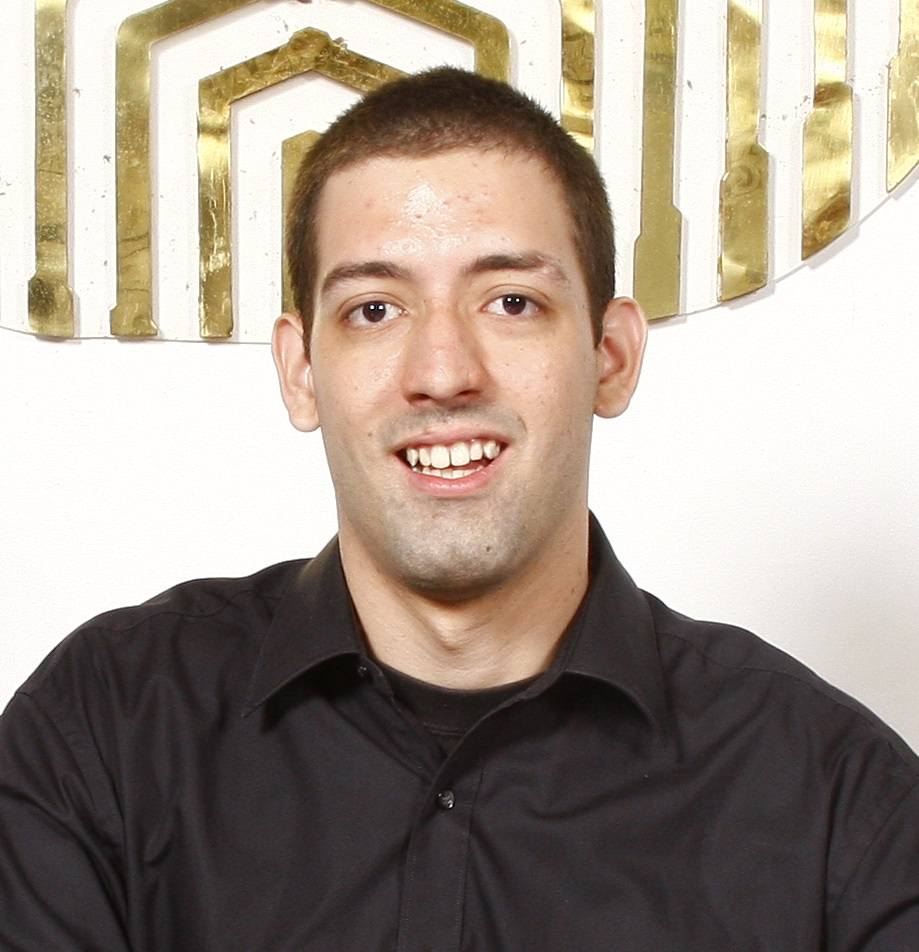
\includegraphics[width=64pt]{picture}}}\\[3mm]
	\@addressstreet, \@addresscity ~~~ \mobilesymbol~\@mobile ~~~ \emailsymbol~\@email
\end{minipage}
\begin{minipage}{70pt}
	
\end{minipage}

Tony lattke Tony lattkeTony lattkeTony lattkeTony lattkeTony lattkeTony lattkeTony lattkeTony lattkeTony lattkeTony lattkeTony lattkeTony lattkeTony lattkeTony lattkeTony lattkeTony lattkeTony lattkeTony lattke

\vfill

\begin{minipage}{1.0\textwidth}
	\section{Inhalt}
	\tableofcontents
\end{minipage}

\newpage
\pagestyle{fancy}
\chapter{Curriculum}{~Vit\ae}
\makequote

%%%%%%%%%%%%%%%%%%%%%%%%%%%%%%%%%%%%%%%%%%%%%%%%%%%%%%%%%%%%%%%%%%%%%%%%%%%%%%%
%									CV
%%%%%%%%%%%%%%%%%%%%%%%%%%%%%%%%%%%%%%%%%%%%%%%%%%%%%%%%%%%%%%%%%%%%%%%%%%%%%%%
\section{Persönliche Daten}

\cvline{Name}{\@firstname~\@secondname~\@familyname~\@secondfamilyname}
\cvline{Anschrift}{\@addressstreet, \@addresscity}
\cvline{Telefon}{\@mobile}
\cvline{E-Mail}{\@email}
\cvline{Geburtsdaten}{14. Februar 1990 in Caracas, Venezuela}
\cvline{Staatsbürgerschaft}{Deutsch und Venezolaner}
\cvline{Familienstand}{Ledig}
\cvline{Website}{\href{http://tonylattke.github.io}{tonylattke.github.io}}
% \cvline{Präsenzdienst}{abgeleistet}
% \cvline{Führerschein}{A,B,C,D,E,F,G}

%%%%%%%%%%%%%%%%%%%%%%%%%%%%%%%%%%%%%%%%%%%%%%%%%%%%%%%%%%%%%%%%%%%%
\section{Ausbildung} 

\cventry{09.2007 -- 09.2013}{Computer-Ingenieur}{Universidad Simón Bolívar}{Venezuela}{\textit{Abschluss}}{}  % arguments 3 to 6 are optional
\cventry{09.2002 -- 07.2007}{Gymnasiast}{U. E. Instituto Humanitas}{Caracas, Venezuela}{\textit{Abschluss}}{} 
%\cventry{xx/xxxx -- xx/xxxx}{Akadem. Grad}{Institution}{Stadt}{\textit{Abschluss}}{Bemerkung} 

%%%%%%%%%%%%%%%%%%%%%%%%%%%%%%%%%%%%%%%%%%%%%%%%%%%%%%%%%%%%%%%%%%%%
% \section{Berufserfahrung} 

% \cventry{xx/xxxx -- xx/xxxx}{Musterkaufmann}{Musterfirma}{Musterort}{}{Bemerkung}

%%%%%%%%%%%%%%%%%%%%%%%%%%%%%%%%%%%%%%%%%%%%%%%%%%%%%%%%%%%%%%%%%%%%
\section{Sprachen} 

\cvline{Spanisch}{Muttersprache}{}
\cvline{Englisch}{Verstehen B2, Sprechen B2, Schreiben B2}
\cvline{Deutsch}{Verstehen A2, Sprechen A2, Schreiben A2}

%\cvline{Englisch}{Verstehen A1, Sprechen B2, Schreiben C3 \hfill {\scriptsize \itshape Europäische Kompetenzstufe}}

%%%%%%%%%%%%%%%%%%%%%%%%%%%%%%%%%%%%%%%%%%%%%%%%%%%%%%%%%%%%%%%%%%%%
\section{Kenntnisse} 

\cvline{Programmier-sprache}{C, C++, C\#, CSS, Haskell, HTML, Java, Javascript, \LaTeX, Matlab, MEL, Perl, PHP, Prolog, Python, R, Ruby, Shell script, SQL}
\cvline{Frameworks}{Catalyst, Django, Rails, XNA, Yesod}
\cvline{Betriebssystem}{Windows, Linux}
\cvline{Software}{3D Studio Max, After Efects, Autocad, Blender, Maya, Photoshop, Unity, Unreal Development Kit, Microsoft Office Word, Excel, PowerPoint, Publisher}
\cvline{Andere}{Git, Heroku}

%%%%%%%%%%%%%%%%%%%%%%%%%%%%%%%%%%%%%%%%%%%%%%%%%%%%%%%%%%%%%%%%%%%%
\section{Kompetenzen} 

\cvline{Caracas Gamejam 2013}{\href{http://globalgamejam.org/2013/enter-panic-heart-attack}{Enter The Panic: Heart Attack}}
\cvline{Caracas Gamejam 2011}{\href{http://archive.globalgamejam.org/2011/enter-panic-attack-matus}{Enter The Panic: The Attack of Matus}}

%%%%%%%%%%%%%%%%%%%%%%%%%%%%%%%%%%%%%%%%%%%%%%%%%%%%%%%%%%%%%%%%%%%%
\section{Universitäre Tätigkeiten} 

\cvline{09.2011 -- 09.2013}{„Leader-Koordinator” in \href{http://joincic.com.ve}{Joincic} (Informatik-Kongress)}
\cvline{09.2012 -- 09.2013}{„Mitarbeiter” in \href{http://usbceic.ldc.usb.ve}{Computer-Ingenieur Studentenzentrum USB}}
\cvline{07.2011 -- 07.2012}{„Präsident” in \href{http://usbceic.ldc.usb.ve}{Computer-Ingenieur Studentenzentrum USB}}
\cvline{09.2010 -- 09.2011}{„Mitarbeiter” in \href{http://joincic.com.ve}{Joincic} (Informatik-Kongress)}
\cvline{09.2010 -- 07.2011}{„Mitarbeiter” in \href{http://usbceic.ldc.usb.ve}{Computer-Ingenieur Studentenzentrum USB}}

%%%%%%%%%%%%%%%%%%%%%%%%%%%%%%%%%%%%%%%%%%%%%%%%%%%%%%%%%%%%%%%%%%%%
\section{Workshops} 

\cvline{VFX Latino América}	{11.2013 -- 02.2014 „Visueller Effekt und 3D Animation”}
\cvline{Instituto Arts}		{09.2011 \hspace{15mm} „After Effects CS5.5”}
\cvline{}					{03.2010 \hspace{15mm} „3D Studio Max 2009 Animation und Entwurf von Zeichen”}
\cvline{}					{12.2009 \hspace{15mm} „3D Studio Max 2009”}
\cvline{}					{08.2006 \hspace{15mm} „Autocad 3D 2006”}
\cvline{}					{07.2005 \hspace{15mm} „Autocad 2D 2006”}
\cvline{Uneweb}				{07.2009 \hspace{15mm} „Blender”}

%%%%%%%%%%%%%%%%%%%%%%%%%%%%%%%%%%%%%%%%%%%%%%%%%%%%%%%%%%%%%%%%%%%%
\section{Fähigkeiten und Fertigkeiten} 

\cvline{}{Proaktive Haltung}
\cvline{}{Ich habe Bereitschaft für neue Fähigkeiten lernen}
\cvline{}{Kreativität und Innovation}
\cvline{}{Die Fähigkeit für Verantwortung übernehmen}
\cvline{}{Die Fähigkeit zur Arbeit in Team}
\cvline{}{Einfach für die Arbeit mit der Öffentlichkeit}

%%%%%%%%%%%%%%%%%%%%%%%%%%%%%%%%%%%%%%%%%%%%%%%%%%%%%%%%%%%%%%%%%%%%
% \section{Interessen}
% \cvline{....}{....}


%%%%%%%%%%%%%%%%%%%%%%%%%%%%%%%%%%%%%%%%%%%%%%%%%%%%%%%%%%%%%%%%%%%%
% \section{Publikationen} 

% \subsection{Konferenzen und Workshops}

% \cvline{mm/jjjj}{Autor 1 und Autor 2. \textbf{Mustertitel: Unser tolles Paper.} In \textit{Proceedings of the First Muster Workshop 1970}, Musterstadt, Musterland, YYYY.}

% \renewcommand*{\refname}{Abschlussarbeiten}
% \nocite{*}
% \bibliographystyle{cv}
% \bibliography{publications}       % 'publications' is the name of a BibTeX file

%%%%%%%%%%%%%%%%%%%%%%%%%%%%%%%%%%%%%%%%%%%%%%%%%%%%%%%%%%%%%%%%%%%%%%%%%%%%%%%
%								Diploma zeugnis
%%%%%%%%%%%%%%%%%%%%%%%%%%%%%%%%%%%%%%%%%%%%%%%%%%%%%%%%%%%%%%%%%%%%%%%%%%%%%%%
\newpage
\chapter{Diploma}{zeugnis}
\vspace*{1cm}
\begin{center}
	Computer-Ingenieur
\end{center}

% Spezialisierung
\cvline{Spezialisierung:}{}
\cvline{}{Computergrafik}
\cvline{}{Künstliche Intelligenz}
\cvline{}{Design und Implementierung von Programmiersprache}

% Wahlfächer
\cvline{Wahlfächer:}{}
\cvline{}{Künstliche Intelligenz für Videospiele}
\cvline{}{Einführung in die Robotik}
\cvline{}{Themen in Computer-Grafiken in Videospielen}

% Thesis Forschungsthema
\cvline{Thesis Forschungsthema:}{}
\cvline{}{Das Projekt erhält eine „Außergewöhnlich gut“ Erwähnung: „Zufällige Inhalt Generator mit Einschränkungen“}

%%%%%%%%%%%%%%%%%%%%%%%%%%%%%%%%%%%%%%%%%%%%%%%%%%%%%%%%%%%%%%%%%%%%%%%%%%%%%%%
%									Master
%%%%%%%%%%%%%%%%%%%%%%%%%%%%%%%%%%%%%%%%%%%%%%%%%%%%%%%%%%%%%%%%%%%%%%%%%%%%%%%

% \newpage
% \chapter{Master}{zeugnis}
% \vspace*{1cm}
% \begin{center}
% 		Test	
% \end{center}

\end{document}